\documentclass[12pt,a4paper]{article}
\documentclass[12pt,a4paper]{article}

%%% Packages %%%
\usepackage{algorithm}		% Algorithms with captions (\begin{algorithm}).
\usepackage{algpseudocode}	% Algorithm pseudocode (\begin{algorithmic}).
\usepackage{amsfonts} 		% For extra mathy stuff (\mathbb).
\usepackage{amsmath} 		% For section headers.
\usepackage{amssymb} 		% For extra mathy stuff, e.g. \therefore.
\usepackage{amsthm}  		% Custom theorem styles.
\usepackage[toc,page]{appendix} % Appendices.
\usepackage{array} 			% Special tabular.
\usepackage{bm}             % Bold, italicised math symbols.
\usepackage{braket} 		% For \set \bra \ket commands.
\usepackage{caption} 		% Caption setup.
\usepackage{centernot} 		% For \centernot.
\usepackage{enumitem} 		% For \setlist.
\usepackage[T1]{fontenc} 	% Code blocks!
\usepackage[margin=1in]{geometry} % global page margin
\usepackage{hyperref} 		% For links.
\usepackage[latin1]{inputenc} % For fancy text input
\usepackage{lipsum} 		% Lorem ipsum <3
\usepackage{listings} 		% Code blocks!
\usepackage{longtable} 		% For the longtable env.
\usepackage{mathtools} 		% \DeclarePairedDelimiter
\usepackage{multirow}		%
\usepackage{scrextend} 		% For the ddmargin env.
\usepackage[inference]{semantic} % Logical inference.
\usepackage{setspace} 		% Custom line spacing.
\usepackage{textcomp} 		% Code blocks.
\usepackage{url} 			% URLs in bibliography.
\usepackage{verbatim} 		% Multiline comments.
\usepackage{wrapfig} 		% Text-wrapping around figures.
\usepackage[svgnames]{xcolor} % For some pretty colours; see https://www.latextemplates.com/svgnames-colors.
\usepackage{ulem}  			% For \sout.

\usepackage{float} % Use [H] instead of [h] to force floats. Works with floats in enumerate/itemize environments.
\usepackage[section]{placeins}  % For floats (figures/tables/algorithms) to be sectioned properly.
% Use \FloatBarrier to mark places where a float shouldn't appear beyond.

\usepackage{graphicx} 		% Graphics~
\graphicspath{{../res/img/}}

\usepackage{booktabs, makecell, tabularx}

% \usepackage{apacite}
\usepackage[sort,comma,nonamebreak]{natbib}
% \bibliographystyle{apalike}
\bibliographystyle{plainnat}
% \bibliographystyle{apacite}


\usepackage{tikz} % Tikz!!!
\usetikzlibrary{arrows}

\usepackage{fancyhdr} % Um... Fancy headers!
\pagestyle{fancy}

% \usepackage{mathptmx} % Times New Romans-esque font.

%%% Tex Commands. %%%

% Side-by-side figures with captions!
% \DeclareCaptionLabelFormat{cont}{#1~#2\alph{ContinuedFloat}}
% \captionsetup[ContinuedFloat]{labelformat=cont}

% Convenience wrapper for bracketing. \delim* for auto-sizing, \delim[\bigg] for manual sizing.
\DeclarePairedDelimiter\ceil{\lceil}{\rceil}
\DeclarePairedDelimiter\floor{\lfloor}{\rfloor}
\DeclarePairedDelimiter\abs{\lvert}{\rvert}
\DeclarePairedDelimiter\parens{(}{)}
\DeclarePairedDelimiter\angles{\langle}{\rangle}

%%%% Useful Macros %%%
\renewcommand{\o}{\varnothing} % Empty set.
\newcommand{\N}{\mathbb{N}} % Natural numbers.
\newcommand{\Z}{\mathbb{Z}} % Integers.
\newcommand{\Q}{\mathbb{Q}} % Rational numbers.
\newcommand{\R}{\mathbb{R}} % Real numbers.
\newcommand{\C}{\mathbb{C}} % Complex numbers.
\newcommand{\powerset}{\mathcal{P}} % Power set.
\newcommand{\insum}{\textstyle\sum} % Inline summation.
\newcommand{\st}{\text{ such that }} % Inline text.
\newcommand{\order}{\text{order}} % Inline summation.
\newcommand{\lcm}{\text{lcm}} % Inline summation.
\newcommand{\Ker}[1]{\text{Ker}\parens*{#1}} % Kernel.

\renewcommand{\epsilon}{\varepsilon}
\renewcommand{\b}[1]{\!\left(#1\right)}

\newcommand{\xor}{\oplus}
\newcommand{\cnot}{\centernot}

\DeclareRobustCommand{\abinom}{\genfrac{\langle}{\rangle}{0pt}{}}

\newcommand{\code}[1]{\texttt{#1}}

\newcommand{\deletecommand}[1]{\let#1\undefined}

% \includecode[<caption>]{filename}
\newcommand{\includecode}[2][]{\lstinputlisting[caption=#1, escapechar=, style=custom_python]{#2}}

\newenvironment{graph}[1]
    {
        \begin{minipage}{#1}
            \centering
            \begin{tikzpicture}
                \tikzset{filled/.style = {shape=circle,fill,minimum size=0.1em}}
                \tikzset{edge/.style = {-,> = latex'}}
                \tikzset{arrow/.style = {->,> = latex'}}
                \tikzset{sibling distance=6em, every node/.style = {shape=circle,draw,minimum size=1em}}
    }
    {
            \end{tikzpicture}
        \end{minipage}
    }

% \newenvironment{tree}[1]
% 	{
% 		\begin{graph}[
% 			sibling distance=10em,
% 			every tree/.style = {shape=rectangle, rounded corners,
% 			  draw, align=center,
% 			  top color=white, bottom color=blue!20}]]
% 			]{#1}
% 	}
% 	{
% 		\end{graph}
% 	}

% Theorems!!!
\newtheorem{theorem}{Theorem}[section]
\newtheorem*{definition*}{Definition}

% Named theorems!
\makeatletter
\newtheoremstyle{namedStyle}
{\topsep}{\topsep}
{}{}
{\bfseries}{.}
{0.5em}
{\thmname{\@ifempty{#3}{#1}\@ifnotempty{#3}{#3}}}
\makeatother
\theoremstyle{namedStyle}
\newtheorem*{solution}{Solution}
\newtheorem*{namedProof}{Proof}

%%% Document Settings %%% 
% Global line spacing.
% \onehalfspacing % 1.5
\doublespacing % 2.0
% \setstretch{1.25} % Custom.

\setlength\parindent{24pt} % Paragraph indent.
\setlength{\headheight}{15pt}

\renewcommand\tabcolsep{5pt} % Table column spacing.
\renewcommand\arraystretch{0.9} % Matrix spacing (or table row spacing).

% Break {align} across pages.
\allowdisplaybreaks


%%% List Settings %%%
% https://tex.stackexchange.com/questions/300340/topsep-itemsep-partopsep-parsep-what-do-they-each-mean-and-what-about

% \setlist{nosep} % Set tight ordered-lists.

% Default enumerate.
\setenumerate{
    label=(\alph*),
    topsep=1pt,
    itemsep=1pt,
    parsep=2pt,
    listparindent=\parindent, % Indents within enumerate.
    }

% \skipitems{n: int}: skip items in an enumerated list
\makeatletter
\newcommand{\skipitems}[1]{%
    \addtocounter{\@enumctr}{#1}%
}
\makeatother

    
%%% Misc. Settings %%%

% Have table and figure use same counter.
\makeatletter 
\let\c@table\c@figure
% \let\c@lstlisting\c@figure
\makeatother

% Graphics.
\graphicspath{ {../res/} }

% Set code format.

%% Usage:
% \begin{lstlisting}[style=custom_python(, options=...)]
% # Code goes here.
% \end{lstlisting}

\lstdefinestyle{custom_python}{
    backgroundcolor = \color{WhiteSmoke},
    basicstyle = \ttfamily\small,
    breaklines = true,
    commentstyle = \itshape\color{DarkGreen},   % Comment style.
    deletekeywords = {set},
    escapeinside = {\%*}{*)},                   % For adding LaTeX in code.
    extendedchars = true,
    frame = single,
    keepspaces = true,
    keywordstyle = \bfseries\color{blue},
    language = Python,                   		% Change the programming language here!
    morekeywords = {*, ValueError, as},
    numbers = left, 							% Line-numbers (possible values: none, left, right).
    numbersep = 10pt,                   		% Distance between line-numbers and code
    numberstyle=\small\color{DarkGray}, 		% Style used for line-numbers.
    rulecolor = \color{black},
    showstringspaces = false,
    stringstyle = \color{red},
    tabsize = 4,
    upquote = true
}

\newcommand{\name}{\textit{redacted}}
\newcommand{\sid}{\textit{redacted}}
\newcommand{\thistitle}{COMP3711 Assignment 3}

\begin{document}
	\lhead{\name}
	\chead{\thistitle}
	\rhead{\sid}

\newpage
\section*{Problem 1}
	
\begin{enumerate}
	\item 
	Algorithm for sorting a $k$-swapped array.\footnote{Inspired by: \url{https://www.geeksforgeeks.org/nearly-sorted-algorithm/}}
	\begin{algorithm}
		\begin{algorithmic}[1]
			\Function{SortKSwapped}{$A$, $n$, $k$}
				\State Create priority queue $q$ of size $k+1$.
				\Comment{$O(1)$}

				\For{$i = 1$ to $k+1$}
				\Comment{Insert the first $k+1$ elements into the p. queue.}

					\State \textproc{Insert}($q$, $A[i]$)
					\Comment{$O(\log k)$}
				\EndFor

				\For{$i = 1$ to $n-k-1$}
				\Comment{Sort the first $n-k-1$ elements.}
					\State $A[i] \gets$ \textproc{ExtractMin}($q$, $k+1$)
					\Comment{$O(\log k)$. Remove and return the min. element.\footnotemark}

					\State \textproc{Insert}($q$, $A[k+i]$)
					\Comment{$O(\log k)$. Insert a new element from the array.}
				\EndFor

				\For{$i = n-k$ to $n$}
				\Comment{Sort the last $k+1$ elements.}
					\State $A[i] \gets$ \textproc{ExtractMin}($q$, $k+1$)
					\Comment{$O(\log k)$}
				\EndFor
			\EndFunction
		\end{algorithmic}
	\end{algorithm}

	\footnotetext{The lecture notes aren't exactly clear on the signature of \textproc{ExtractMin}. I've taken the liberty to express it as a function that takes the p. queue $q$ and the size of the queue $k+1$, and returns the minimum element (before removal).}

	The algorithm first creates a priority queue of $k+1$ elements. This yields \textproc{Insert} and \textproc{ExtractMin} operations of $O(\log k)$ complexity. We initialise the queue by inserting the first $k+1$ elements of $A$.

	We then get to the fun part... sorting. This is split into two loops. The first loop sorts the first $n-k-1$ elements \textit{and} inserts the remaining $n-k-1$ elements of the array (alternating between extract and insert each iteration). The second loop sorts the last $k+1$ elements.

	And the array is sorted.

	\item
	Note that the $1$-st smallest element is within $A[max(1,i-k) \dots min(n,i+k)]$. Since the priority queue $q$ can hold up to $k+1$ elements, so the $i$-th time we extract, we get the $i$-th smallest element of the entire array. We do this for the whole array and take care to insert the remaining elements at the same time as sorting the front (in the second loop).

	\item
	Note that although the heap operations actually take $O(\log (k + 1))$, we simplify this to $O(\log k)$.

	The first loop (lines 3-5) takes $O(k \log k)$ time since it runs $k$ iterations of an $O(\log k)$ operation (\textproc{Insert}).
	The second loop takes $O(2(n-k)\log k)$ time since it runs $n - k$ iterations of two $O(\log k)$ operations (\textproc{ExtractMin} followed by \textproc{Insert}).
	The final loop takes $O(k \log k)$ operations since it runs $k$ iterations of an $O(\log k)$ operation (\textproc{ExtractMin}).

	Altogether, \textproc{SortKSwapped} runs in $O(k \log k + 2(n-k)\log k + k \log k) = O(n \log k)$ time.

	\item
	The comparison-based algorithm makes no assumptions on the elements of the array and assumes $n!$ leaves in the decision tree. With a $k$-swapped array, it is assumed that $A[i] < A[k+i]$ for all $1 \le i \le n-k$, so this eliminates some leaves in the decision tree and is what allows us to use a priority queue of size $k$ instead of $n$.

	\item 
	We can separate the array into blocks of less than or equal to $k$. These blocks are localised and all elements in one block are smaller than all elements in the next block. The lower bound of leaves is then $(k!)^{n/k}$ which yields $\Omega(n \log k)$ by Stirling's approximation.

\end{enumerate}


\newpage
\section*{Problem 2}

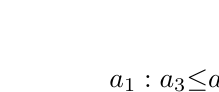
\begin{tikzpicture}[every tree node/.style={draw,circle},
	level distance=1.25cm,sibling distance=.5cm, 
	edge from parent path={(\tikzparentnode) -- (\tikzchildnode)}]
\Tree [.{$a_1 : a_3$}
	\edge node[auto=right] {$\le$};  
	[.{$a_2 : a_3$}
		\edge node[auto=right] {$\le$};
		[.\node[shape=rectangle] {$a_1, a_2, a_3, a_4$};]
		\edge node[auto=left] {$>$};
		[.{$a_2 : a_4$}
			\edge node[auto=right] {$\le$};
			[.\node[shape=rectangle] {$a_1, a_3, a_2, a_4$};]
			\edge node[auto=left] {$>$};
			[.\node[shape=rectangle] {$a_1, a_3, a_4, a_2$};]
		]
	]
	\edge node[auto=left] {$>$};
	[.{$a_1 : a_4$}
		\edge node[auto=right] {$\le$};
		[.{$a_2 : a_4$}
			\edge node[auto=right] {$\le$};
			[.\node[shape=rectangle] {$a_3, a_1, a_2, a_4$};]
			\edge node[auto=left] {$>$};
			[.\node[shape=rectangle] {$a_3, a_1, a_4, a_2$};]
		]
		\edge node[auto=left] {$>$};
		[.\node[shape=rectangle] {$a_3, a_4, a_1, a_2$};]
	]
]
\end{tikzpicture}

\newpage
\section*{Problem 3}

\begin{enumerate}
	\item 
	\begin{align*}
		[29681, 53846, 43521, 39427, 32433, 35700, 30764, 16892, 52608, 19583] \\
		[35700, 29681, 43521, 16892, 32433, 19583, 30764, 53846, 39427, 52608] \\
		[35700, 52608, 43521, 39427, 32433, 53846, 30764, 29681, 19583, 16892] \\
		[39427, 32433, 43521, 19583, 52608, 29681, 35700, 30764, 53846, 16892] \\
		[30764, 32433, 52608, 43521, 53846, 35700, 16892, 39427, 19583, 29681] \\
		[16892, 19583, 29681, 30764, 32433, 35700, 39427, 43521, 52608, 53846]
	\end{align*}

	\item 
	\begin{align*}
		[8b74, 73f1, aa01, 41fc, 7eb1, 4c7f, 782c, d256, 9a03, cd80] \\
		[cd80, 73f1, aa01, 7eb1, 9a03, 8b74, d256, 41fc, 782c, 4c7f] \\
		[aa01, 9a03, 782c, d256, 8b74, 4c7f, cd80, 7eb1, 73f1, 41fc] \\
		[41fc, d256, 73f1, 782c, aa01, 9a03, 8b74, 4c7f, cd80, 7eb1] \\
		[41fc, 4c7f, 73f1, 782c, 7eb1, 8b74, 9a03, aa01, cd80, d256] \\
	\end{align*}
\end{enumerate}


\newpage
\section*{Problem 4}

\begin{enumerate}
	\item
	We sort the input by the endpoints $f_j$ then use induction to show that a minimal $A \subseteq \{f_1, \dots, f_n\}$ exists.

	By induction, suppose we have the base case of one interval $I_1$. Trivially, $\{f_1\}$ is a minimal cover. Now assume that the first $k$ intervals can be minimally covered by some $A \subseteq \{f_1, \dots, f_k\}$.
	
	We now introduce the $k+1$-th interval, $I_{k+1}$. Since we've sorted the input by the endpoints, so $f_k \le f_{k+1}$. There are two cases, either $I_{k+1}$ does not overlap with any previous intervals, or it does overlap with some. If it doesn't overlap, then we simply add $f_{k+1}$ to $A$ so that $I_{k+1}$ is covered. On the other hand, if it does overlap, then there exists a set of endpoints $J$ such that $f_j \in I_{k+1}$ for all $f_j \in J$. If none of $f_j$ are in $A$ (i.e. $J \cap A = \o$), then we add $f_{k+1}$ to $A$; otherwise, $A$ already covers $I_{k+1}$.
	
	In any circumstance, $A$ now remains a minimal cover and $A \subseteq \{f_1, \dots, f_{k+1}\}$. Thus there exists a minimal cover $A$ such that $A \subseteq \{f_1, \dots, f_{k+1}\}$.

	\item \-\\
	\begin{algorithm}
		\begin{algorithmic}[1]
			\Function{GreedyCovering}{$I$, $n$}
				\State Sort intervals by $f_i$.
				\Comment{$O(n \log n)$ worst case complexity.}

				\State $A \gets \o$
				\State $j \gets 1$
				\While{$j \le n$}
					\State $t \gets I[j].f$
					\Comment{Get the endpoint $f_j$}

					\State $A \gets A \cup \{t\}$
					\Comment{Add $f_j$ to the covering}

					\State $j \gets j + 1$
					\Comment{Skip this interval, we know it covers}

					\While{$j \le n$ \textbf{and} $I[j].s \le t$ \textbf{and} $t \le I[j].f$}
					\Comment{Advance while $t$ can cover $I[j]$}
						\State $j \gets j + 1$
					\EndWhile
				\EndWhile
				\Return $A$
			\EndFunction
		\end{algorithmic}
	\end{algorithm}

	\newpage
	\item
	Suppose that our greedy solution (\textproc{Greedy}) is not optimal and there exists an optimal solution (\textproc{Opt}).
	
	We collect the times returned by each solution. Let $g = \angles{g_1, \dots, g_m}$ and $h = \angles{h_1, \dots, h_n}$ be sorted arrays containing the points returned by \textproc{Greedy} and \textproc{Opt} respectively (with $n < m$).

	For the base case of $i = 1$, since $g_1$ is an endpoint, so $h_1 \le g_1$. (If $h_1 > g_1$, then $h_1$ won't cover $I_1$.) Now assume that the first $j$ intervals have been covered by $k$ points ($k < n < m$), and consider the next interval $I_{j+1}$ with points $g_{k+1}$ and $h_{k+1}$. The situation repeats as with the base case. It is imperative that $h_{k+1} \le g_{k+1}$, otherwise $I_{j+1}$ won't be covered. In the end, we have $n = m$, contradicting our initial assumption that \textproc{Greedy} is not optimal. Thus \textproc{Greedy} is optimal.
	
	\item
	The time complexity is bounded by sorting. The rest of the code is just a loop that runs in $O(n)$ time. Each interval is only considered once. Each interval is either added (lines 6-8) or was covered (lines 9) by some previous finish time.

\end{enumerate}

\newpage
\section*{Problem 5}

\begin{enumerate}
	\item \-\\
	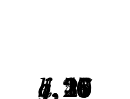
\begin{tikzpicture}[every tree node/.style={draw,circle},
		level distance=1.25cm,sibling distance=.5cm, 
		edge from parent path={(\tikzparentnode) -- (\tikzchildnode)}]
	\Tree [.{}
		\edge node[auto=right] {0};
		[.{}
			\edge node[auto=right] {0};
			[.\node[shape=rectangle] {$c,58$};]
			\edge node[auto=left] {1};
			[.{}
				\edge node[auto=right] {0};
				[.\node[shape=rectangle] {$f,29$};]
				\edge node[auto=left] {1};
				[.{}
					\edge node[auto=right] {0};
					[.\node[shape=rectangle] {$d,16$};]
					\edge node[auto=left] {1};
					[.\node[shape=rectangle] {$e,17$};]
				]
			]
		]
		\edge node[auto=left] {1};
		[.{}
			\edge node[auto=right] {0};
			[.{}
				\edge node[auto=right] {0};
				[.\node[shape=rectangle] {$a,36$};]
				\edge node[auto=left] {1};
				[.\node[shape=rectangle] {$g,45$};]
			]
			\edge node[auto=left] {1};
			[.{}
				\edge node[auto=right] {0};
				[.{}
					\edge node[auto=right] {0};
					[.\node[shape=rectangle] {$b,21$};]
					\edge node[auto=left] {1};
					[.\node[shape=rectangle] {$i,26$};]
				]
				\edge node[auto=left] {1};
				[.{}
					\edge node[auto=right] {0};
					[.\node[shape=rectangle] {$h,27$};]
					\edge node[auto=left] {1};
					[.\node[shape=rectangle] {$j,28$};]
				]
			]
		]
	]
	\end{tikzpicture}

	\item
	\begin{tabular}[h!]{|r|l|}
		\hline
		$a$ & 100 \\
		$b$ & 1100 \\
		$c$ & 00 \\
		$d$ & 0110 \\
		$e$ & 0111 \\
		$f$ & 010 \\
		$g$ & 101 \\
		$h$ & 1110 \\
		$i$ & 1101 \\
		$j$ & 1111 \\
		\hline
	\end{tabular}

	\item
	\begin{tabular}[h!]{|r|l|}
		\hline
		$c$ & 00 \\
		$a$ & 100 \\
		$f$ & 010 \\
		$g$ & 101 \\
		$b$ & 1100 \\
		$d$ & 0110 \\
		$e$ & 0111 \\
		$h$ & 1110 \\
		$i$ & 1101 \\
		$j$ & 1111 \\
		\hline
	\end{tabular}
	

\end{enumerate}

\end{document}